\documentclass{article}
\usepackage{fullpage}
%%% Работа с русским языком
\usepackage[T2A]{fontenc}
\usepackage[utf8]{inputenc}
\usepackage[english,russian]{babel}   %% загружает пакет многоязыковой вёрстки
%\usepackage{fontspec}      %% подготавливает загрузку шрифтов Open Type, True Type и др.
%\defaultfontfeatures{Ligatures={TeX},Renderer=Basic}  %% свойства шрифтов по умолчанию
%\setmainfont[Ligatures={TeX,Historic}]{Times New Roman} %% задаёт основной шрифт документа
%\setsansfont{Comic Sans MS}                    %% задаёт шрифт без засечек
%\setmonofont{Courier New}
\usepackage{indentfirst}
\frenchspacing
\usepackage{graphicx}
\usepackage{titlesec} % package to customize chapters, sections and subsections style
%--------------------------------------
\titleformat{\section}{\large\bfseries\centering}{\thesection}{1em}{}
%Hyphenation rules
%--------------------------------------
\usepackage{hyphenat}
\hyphenation{мате-мати-ка восста-навливать}
%--------------------------------------
%%% Дополнительная работа с математикой
\usepackage[intlimits,sumlimits]{amsmath}
\usepackage{amsfonts,amssymb,amsthm,mathtools} % AMS
%\usepackage{amsmath,amsfonts,amssymb,amsthm,mathtools} % AMS
\usepackage{icomma} % "Умная" запятая: $0,2$ --- число, $0, 2$ --- перечисление

%% Перенос знаков в формулах (по Львовскому)
\newcommand*{\hm}[1]{#1\nobreak\discretionary{}
{\hbox{$\mathsurround=0pt #1$}}{}}

\renewcommand{\le}{\ensuremath{\leqslant}}
\renewcommand{\leq}{\ensuremath{\leqslant}}
\renewcommand{\ge}{\ensuremath{\geqslant}}
\renewcommand{\geq}{\ensuremath{\geqslant}}

\title{Контрольная работа}
\author{Теория вероятностей и математическая статистика}
\date{Декабрь 2015}

\begin{document}

\maketitle
\section*{Вариант № 2.}
\begin{enumerate}

\item % Задание 1
В ящике 20 белых и 30 чёрных шаров. Наудачу взяли 10 шаров. Какова вероятность того, что среди них 5 белых шаров.
\begin{center}Решение:\end{center}
Перенумеруем все шары. Всего шаров 50 штук. Исходом считаем выбор 10 любых шаров.
Количество всех исходов равно
$$n=C_{50}^{10}=\frac{50!}{10!\cdot40!}=\frac{41\cdot42\cdot43\cdot44\cdot45\cdot46\cdot47\cdot48\cdot49\cdot50}{1\cdot2\cdot3\cdot4\cdot5\cdot6\cdot7\cdot8\cdot9\cdot10}=41\cdot43\cdot11\cdot46\cdot47\cdot49\cdot5=10272278170$$
Благоприятный исход - выбор 5 белых шаров и 5 чёрных. \newline
5 белых шаров из 20 можно выбрать $C_{20}^{5}$ способами. А выбрать 5 чёрных шаров из 30 можно $C_{30}^{5}$ способами. \newline
Количество благоприятных исходов равно произведению
$$m=C_{20}^{5}\cdot C_{30}^{5}=\frac{20!}{5!\cdot15!}\cdot\frac{30!}{5!\cdot25!}=\frac{16\cdot17\cdot18\cdot19\cdot20}{1\cdot2\cdot3\cdot4\cdot5}\cdot\frac{26\cdot27\cdot28\cdot29\cdot30}{1\cdot2\cdot3\cdot4\cdot5}=$$
$$=(16\cdot17\cdot3\cdot19)\cdot(26\cdot27\cdot7\cdot29)=15504\cdot142506=2209413024$$
$$P=\frac{m}{n}=\frac{2209413024}{10272278170}\approx0,215$$

Ответ: $\approx0,215$.

\item % Задание 2
В партии товаров товаровед отбирает бракованные изделия. Вероятность того, что наудачу взятое изделие окажется бракованным, равна $0,1$. Найти вероятность того, что из трёх взятых на проверку изделий одно бракованное.
\begin{center}Решение:\end{center}
В этой задаче мы имеем дело с серией независимых испытаний, так что здесь применима формула Бернулли:
$$P_3(1)=C_3^1\cdot0,1^1\cdot0,9^2=3\cdot0,1\cdot0,81=0,243$$
Но если её не использовать, то можно рассуждать так: \newline
Будем считать исходом выбор трёх произольных изделий. Благоприятным исходом будем считать исход при котором одно бракованное изделие, а два остальные не бракованные. Таких исходов может быть всего три: когда бракованным оказалось первое, когда бракованным оказалось второе, и наконец, когда бракованным оказалось третье.
$$P=0,1\cdot0,9\cdot0,9+0,9\cdot0,1\cdot0,9+0,9\cdot0,9\cdot0,1=3\cdot0,081=0,243$$

Ответ: $0,243$.

\item % Задание 3
В двух ящиках содержится по 20 деталей, причём стандартных деталей в первом ящике 13, а во втором 18, из второго ящика извлечена одна деталь, и переложена в первый ящик. После этого из первого ящика извлечена деталь, оказавшаяся стандартной. Найти вероятность того, что из второго ящика в первый была переложена стандартная деталь.
\begin{center}Решение:\end{center}
Пусть $H_1$, $H_2$ - гипотезы по поводу того, была ли перекладываемая деталь стандартной или нет соответственно. \newline Тогда вероятности этих гипотез $P(H_1)=\frac{18}{20}=0,9$ и $P(H_2)=\frac{2}{20}=0,1$ находятся по формуле классической вероятности, отношением числа стандартных (и соответственно нестандартных) деталей во втором ящике к общему числу деталей во втором ящике.  \newline Пусть событие $A$ заключается в том, что извлечённая из второго ящика деталь оказалась стандартной. \newline
Так же по формуле классической вероятности находятся вероятности $P(A/H_1)=\frac{13+1}{21}=\frac{2}{3}$ и $P(A/H_2)=\frac{13}{21}$ извлечения стандартной детали уже из первого ящика, после того как общее количество деталей в нём увеличилось на 1. \newline
Теперь для нахождения искомой $P(H_1/A)$ применим формулу Байеса:

$$P(H_1/A)=\frac{P(H_1)P(A/H_1)}{P(H_1)P(A/H_1)+P(H_2)P(A/H_2)}=\frac{0,9\cdot\frac{2}{3}}{0,9\cdot\frac{2}{3}+0,1\cdot\frac{13}{21}}=\frac{0,6}{\frac{13,9}{21}}=\frac{12,6}{13,9}\approx0,9.$$

Ответ: $\approx0,9$.

\item % Задание 4
Найти вероятность того, что в $n$ независимых испытаний событие появится не менее $k$ раз, зная, что в каждом испытании вероятность появления события равна $p$.

$$n=5; k=2; p=0,2.$$
\begin{center}Решение:\end{center}
Используем формулу Бернулли $P_n(k)=C_n^k p^k q^{n-k}$, вероятность того, что событие наступит не менее $k$ раз с помощью неё вычисляется так: $$P_n(i\ge k)=\sum_{i=k}^n P_n(i)$$
В нашем случае $n=5; k=2; p=0,2; q=0,8;$ значит
$$P_5(i\ge 2)=\sum_{i=2}^5 P_5(i)=P_5(2)+P_5(3)+P_5(4)+P_5(5)=C_5^2\cdot0,2^2\cdot0,8^3+C_5^3\cdot0,2^3\cdot0,8^2+$$
$$+C_5^4\cdot0,2^4\cdot0,8+C_5^5\cdot0,2^5=10\cdot0,04\cdot0,512+10\cdot0,008\cdot0,64+5\cdot0,0016\cdot0,8+0,00032=$$
$$=0,2048+0,0512+0,0064+0,00032=0,26272.$$

Ответ: $0,26272$.

\item % Задание 5
Найти а) математическое ожидание; б) дисперсию; в) среднее квадратическое отклонение дискретной случайной величины $X$ по закону её распределения, заданному рядом распределения (в первой строке таблицы указаны возможные значения, во второй строке - вероятности возможных значений).

\begin{center}
\begin{tabular}{|c|c|c|c|c|c|}
\hline
$X$ & 10 & 13 & 17 & 19 & 22 \\
\hline
$p$ & $0,2$ & $0,1$ & $0,2$ & $0,4$ & $0,1$ \\
\hline
\end{tabular}
\end{center}
\begin{center}Решение:\end{center}
а) Математическое ожидание: $$M(X)=\sum_{i=1}^n x_i p_i=10\cdot0,2+13\cdot0,1+17\cdot0,2+19\cdot0,4+22\cdot0,1=2+1,3+3,4+7,6+2,2=16,5.$$
б) Дисперсия:
$$D(X)=\sum_{i=1}^n (x_i-m)^2 p_i=(10-16,5)^2\cdot0,2+(13-16,5)^2\cdot0,1+(17-16,5)^2\cdot0,2+(19-16,5)^2\cdot0,4+$$
$$+(22-16,5)^2\cdot0,1=6,5^2\cdot0,2+3,5^2\cdot0,1+0,5^2\cdot0,2+2,5^2\cdot0,4+5,5^2\cdot0,1=15,25.$$
в) Среднее квадратическое отклонение:
$$\sigma=\sqrt{D(X)}=\sqrt{15,25}\approx3,9.$$

Ответ: а)$16,5$; б)$15,25$; в)$\approx3,9$.

\item % Задание 6
Случайная величина $X$ задана функцией распределения $F(x)$. Найти плотность распределения вероятностей, математическое ожидание, дисперсию случайной величины и построить графики $f(x)$ и $F(x)$.

\begin{equation*}
F(x) =
 \begin{cases}
  0, & x\leq0\\
  (x^2-x)/2, & 0<x\leq1\\
  1, & x>1
 \end{cases}
\end{equation*}
\begin{center}Решение:\end{center}
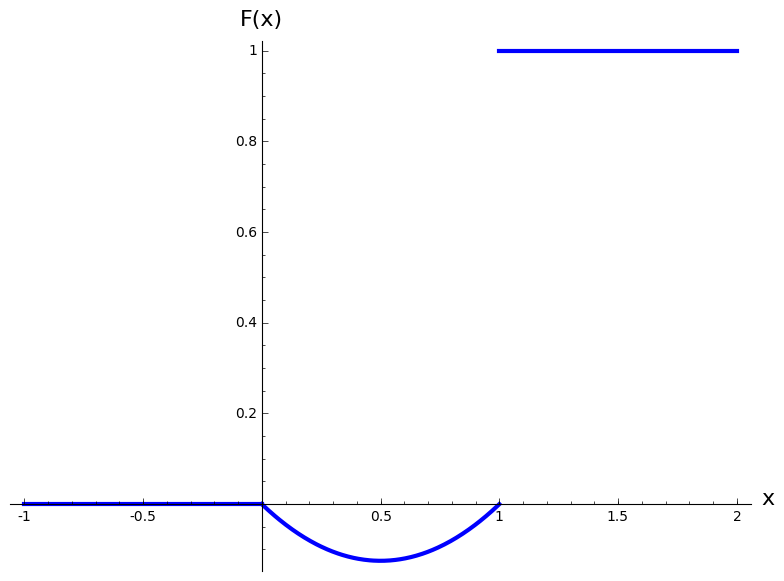
\includegraphics[width=340pt,natwidth=784,natheight=581]{2_6_1.png}
\begin{equation*}
f(x) = F^{\prime}(x) =
 \begin{cases}
  0, & x\leq0\\
  x-\frac{1}{2}, & 0<x\leq1\\
  0, & x>1
 \end{cases}
\end{equation*}
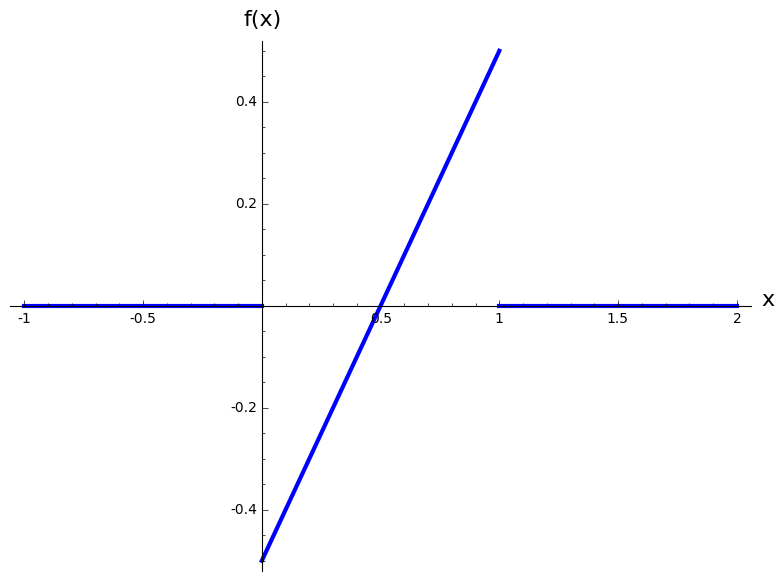
\includegraphics[width=340pt,natwidth=784,natheight=581]{2_6_2.png}
$$m=M(X)=\int_{-\infty}^{+\infty} x f(x) dx=\int_{0}^{1} x\left(x-\frac{1}{2}\right) dx=\int_{0}^{1} x^2dx - \frac{1}{2}\int_{0}^{1} xdx=\left(\frac{x^3}{3}-\frac{x^2}{4}\right)\bigg|_{0}^{1}=\frac{1}{12}\approx0,08.$$
$$D(X)=\int_{-\infty}^{+\infty} (x-m)^2 f(x) dx=\int_{0}^{1} \left(x-\frac{1}{12}\right)^2\left(x-\frac{1}{2}\right) dx=\int_{0}^{1} \left(x^3-\frac{2x^2}{3}+\frac{13x}{144}-\frac{1}{288}\right) dx=$$
$$=\left(\frac{x^4}{4}-\frac{2x^3}{9}+\frac{13x^2}{288}-\frac{x}{288}\right)\bigg|_{0}^{1}=\frac{1}{4}-\frac{2}{9}+\frac{13}{288}-\frac{1}{288}=\frac{5}{72}\approx0,07.$$



\item % Задание 7
Заданы математическое ожидание $m$ и среднее квадратическое отклонение $\sigma$ нормально распределённой случайной величины. \newline
Требуется найти: а) вероятность того, что $X$ примет значение, принадлежащее интервалу $(a, b)$; \newline
б) вероятность того, что абсолютная величина отклонения $|X-m|$ окажется меньше положительного числа $n$.

$$m=7;\sigma=3;a=3;b=13;n=6$$
\begin{center}Решение:\end{center}
а) $$P(a<X<b)=\Phi\left(\frac{b-m}{\sigma}\right)-\Phi\left(\frac{a-m}{\sigma}\right)=\Phi\left(\frac{13-7}{3}\right)-\Phi\left(\frac{3-7}{3}\right)=$$
$$=\Phi(2)+\Phi\left(\frac{4}{3}\right)=0,47725+0,40824=0,88549.$$
б)
$$P (|X-m| < n)= 2\Phi\left(\frac{n}{\sigma}\right)=2\Phi\left(\frac{6}{3}\right)=2\cdot0,47725=0,9545.$$

Ответ: а)$0,88549$; б)$0,9545$.

\item % Задание 8
Дано статическое распределение выборки (в первой строке указаны выборочные варианты $x_j$, а во второй строке - соответствующие частоты).

Требуется:

1) Построить полигон частот.

2) Найти выборочнуюсреднюю $x_\textit{в}$ (несмещённую оценку средней)

3) Найти выборочную дисперсию (смещённую оценку)

4) Найти <<Исправленную>> выборочную дисперсию $S^2$ (несмещённую оценку) и <<исправленное>> среднее квадратическое отклонение $S$.

\begin{center}
\begin{tabular}{|c|c|c|c|c|c|c|c|}
\hline
$x_j$ & 100 & 140 & 150 & 170 & 180 & 190 & 200 \\
\hline
$n_j$ & 10 & 15 & 40 & 35 & 20 & 10 & 5 \\
\hline
\end{tabular}
\end{center}
\begin{center}Решение:\end{center}
1) Найдем сначала объём выборки: $$n=\sum_{j=1}^k n_j=10+15+40+35+20+10+5=135$$

Полигон частот:

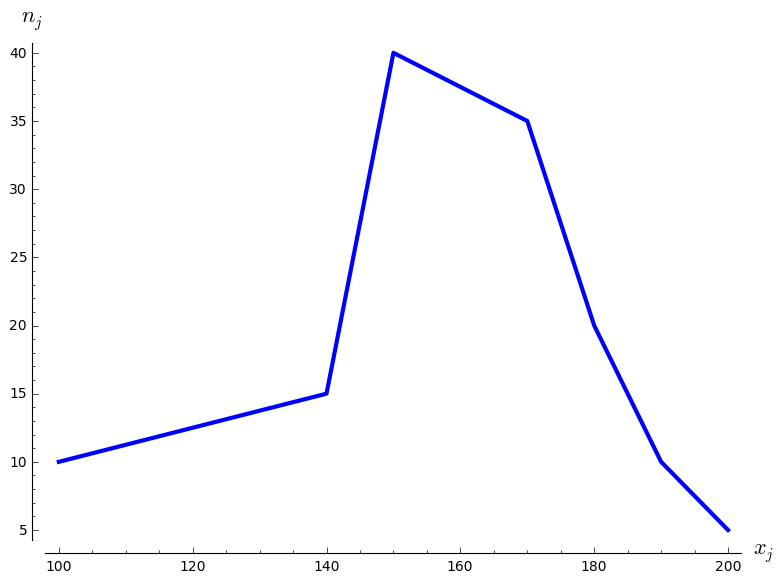
\includegraphics[width=340pt,natwidth=783,natheight=583]{2_8.png}

2) Выборочная средняя:
$$\overline{x_\textit{в}}=\frac{1}{n}\sum_{j=1}^k n_j x_j=\frac{1}{135}\cdot\left(10\cdot100+15\cdot140+40\cdot150+35\cdot170+20\cdot180+10\cdot190+5\cdot200\right)=$$
$$=\frac{21550}{135}=\frac{4310}{27}\approx159,63.$$

3) Выборочная дисперсия:
\begin{multline*}
D_{\textit{в}}=\frac{1}{n}\sum_{j=1}^k n_j
\cdot\left(x_j-\overline{x_\textit{в}}\right)^2=
\frac{1}{135}\cdot\left(10\cdot\left(100-\frac{4310}{27}\right)^2+15\cdot\left(140-\frac{4310}{27}\right)^2+40\cdot\left(150-\frac{4310}{27}\right)^2+\right.\\
+\left.35\cdot\left(170-\frac{4310}{27}\right)^2+20\cdot\left(180-\frac{4310}{27}\right)^2+10\cdot\left(190-\frac{4310}{27}\right)^2+5\cdot\left(200-\frac{4310}{27}\right)^2\right)=\\
=\frac{1}{135\cdot27^2}\cdot\left(10\cdot1610^2+15\cdot530^2+40\cdot260^2+35\cdot280^2+20\cdot550^2+10\cdot820^2+5\cdot1090^2\right)=\\
=\frac{100}{98415}\cdot\left(10\cdot25921+15\cdot2809+40\cdot676+35\cdot784+20\cdot3025+10\cdot6724+5\cdot11881\right)=
\end{multline*}
$$=\frac{54297000}{98415}\approx551,7.$$
4) <<Исправленная>> выборочная дисперсия:
$$S^2=\frac{n}{n-1}D_{\textit{в}}=\frac{54297000}{134\cdot27^2}\approx555,83.$$
<<Исправленное>> среднее квадратическое отклонение:
$$S=\sqrt{S^2}=\sqrt{\frac{54297000}{134\cdot27^2}}\approx23,576$$

\item % Задание 9
Найти доверительные интервалы для оценки математического ожидания с надёжностью $\gamma=0,95$; зная выборочную среднюю $\overline{x_\textit{в}}$, объём выборки $n$ и среднее математическое отклонение $\sigma$ нормально распределенной величины $X$.

$$\overline{x_\textit{в}}=175,16; \sigma=8; n=64.$$
\begin{center}Решение:\end{center}
$$\overline{x_\textit{в}}-t\cdot\left(\frac{\sigma}{\sqrt{n}}\right)<m<\overline{x_\textit{в}}+t\cdot\left(\frac{\sigma}{\sqrt{n}}\right)$$
Значению функции Лапласа $\Phi(t)=\frac{\gamma}{2}=\frac{0,95}{2}=0,475$ соответствует $t=1,96$.

Теперь мы знаем всё для того чтобы найти доверительный интервал для оценки математического ожидания:
$$175,16-1,96\cdot\left(\frac{8}{\sqrt{64}}\right)<m<175,16+1,96\cdot\left(\frac{8}{\sqrt{64}}\right);$$
$$175,16-1,96<m<175,16+1,96;$$
$$173,2<m<177,12.$$
Ответ: $(173,2;177,12)$.

\end{enumerate}

\section*{Вариант № 4.}
\begin{enumerate}

\item % Задание 1
В ящике 50 деталей, из которых 10 бракованных. Наудачу взяли 8 деталей. Какова вероятность того, что среди них 2 детали бракованные.
\begin{center}Решение:\end{center}
Перенумеруем все детали. Исходом считаем выбор 8 любых деталей.
Количество всех исходов равно
$$n=C_{50}^{8}=\frac{50!}{8!\cdot42!}=\frac{43\cdot44\cdot45\cdot46\cdot47\cdot48\cdot49\cdot50}{1\cdot2\cdot3\cdot4\cdot5\cdot6\cdot7\cdot8}=43\cdot11\cdot3\cdot23\cdot47\cdot7\cdot50=536878650$$
Благоприятный исход - выбор двух бракованных деталей и 6 небракованных. \newline
2 бракованные детали из 10 можно выбрать $C_{10}^{2}$ способами. А выбрать 6 небракованных деталей из 40 можно $C_{40}^{6}$ способами. \newline
Количество благоприятных исходов равно произведению
$$m=C_{10}^{2}\cdot C_{40}^{6}=\frac{10!}{2!\cdot8!}\cdot\frac{40!}{6!\cdot34!}=\frac{9\cdot10}{2}\cdot\frac{35\cdot36\cdot37\cdot38\cdot39\cdot40}{1\cdot2\cdot3\cdot4\cdot5\cdot6}=$$
$$=45\cdot(35\cdot37\cdot38\cdot39\cdot2)=45\cdot3838380=172727100$$
$$P=\frac{m}{n}=\frac{172727100}{536878650}\approx0,32$$

Ответ: $\approx0,32$.

\item % Задание 2
Вероятность хотя бы одного попадания в цель при залпе из двух орудий равна $0,92$. Найти вероятность попадания в цель первым орудием, если вероятность попадания вторым орудием равна $0,8$.
\begin{center}Решение:\end{center}
Обозначим за $p$ вероятность попадания в цель первым орудием. Тогда вероятность того что оба орудия промхнутся при залпе $(1-p)\cdot(1-0,8)=(1-p)\cdot0,2$. С другой стороны это событие будет являться дополнением того события что хоть одно орудие попало в цель, значит его вероятность $1-0,92=0,08$. \newline Имеем уравнение:
$(1-p)\cdot0,2=0,08$;
$1-p=\frac{0,08}{0,2}$;
$p=1-\frac{0,08}{0,2}=1-0,4=0,6$.

Ответ: $0,6$.

\item % Задание 3
Сборщик получил две коробки одинаковых деталей, изготовленных заводом $N_1$, и три коробки таких же деталей, изготовленных заводом $N_2$. Вероятность того, что деталь заводов $N_1$ и $N_2$ стандартная, равна соответственно $0,9$ и $0,8$. Из наудачу взятой коробки сборщик взял деталь, которая оказалась стандартной. Определить вероятность того, что взятая деталь изготовлена заводом $N_1$.
\begin{center}Решение:\end{center}
Всего имеется 5 коробок с деталями, и надо полагать что в коробках одинаковое количество деталей. \newline
Пусть $H_1$, $H_2$ - гипотезы по поводу того, была взятая деталь изготовлена заводом $N_1$ или заводом $N_2$ соответственно. \newline Тогда вероятности этих гипотез $P(H_1)=\frac{2}{5}=0,4$ и $P(H_2)=\frac{3}{5}=0,6$ находятся по формуле классической вероятности как отношение числа коробок с соответствующего завода на общее число коробок. \newline Пусть событие $A$ заключается в том, что извлечённая из наудачу взятой коробки деталь оказалась стандартной. \newline
Из условия задачи мы знаем вероятности $P(A/H_1)=0,9$ и $P(A/H_2)=0,8$ извлечения стандартной детали из ящиков произведенных заводами $N_1$ и $N_2$ соответственно. \newline
Теперь для нахождения искомой $P(H_1/A)$ применим формулу Байеса:

$$P(H_1/A)=\frac{P(H_1)P(A/H_1)}{P(H_1)P(A/H_1)+P(H_2)P(A/H_2)}=\frac{0,4\cdot0,9}{0,4\cdot0,9+0,6\cdot0,8}=\frac{0,36}{0,36+0,48}=\frac{0,36}{0,84}\approx0,43.$$
Ответ: $\approx0,43$.

\item % Задание 4
Найти вероятность того, что в $n$ независимых испытаний событие появится не менее $k$ раз, зная, что в каждом испытании вероятность появления события равна $p$.

$$n=5; k=2; p=0,4.$$
\begin{center}Решение:\end{center}
Используем формулу Бернулли $P_n(k)=C_n^k p^k q^{n-k}$, вероятность того, что событие наступит не менее $k$ раз с помощью неё вычисляется так: $$P_n(i\ge k)=\sum_{i=k}^n P_n(i)$$
В нашем случае $n=5; k=2; p=0,4; q=0,6;$ значит
$$P_5(i\ge 2)=\sum_{i=2}^5 P_5(i)=P_5(2)+P_5(3)+P_5(4)+P_5(5)=C_5^2\cdot0,4^2\cdot0,6^3+C_5^3\cdot0,4^3\cdot0,6^2+$$
$$+C_5^4\cdot0,4^4\cdot0,6+C_5^5\cdot0,4^5=10\cdot0,16\cdot0,216+10\cdot0,064\cdot0,36+5\cdot0,0256\cdot0,6+0,01024=$$
$$=0,3456+0,2304+0,0768+0,01024=0,66304.$$

Ответ: $0,66304$.

\item % Задание 5
Найти а) математическое ожидание; б) дисперсию; в) среднее квадратическое отклонение дискретной случайной величины $X$ по закону её распределения, заданному рядом распределения (в первой строке таблицы указаны возможные значения, во второй строке - вероятности возможных значений).

\begin{center}
\begin{tabular}{|c|c|c|c|c|c|}
\hline
$X$ & $1,4$ & $2,2$ & $3,5$ & $4,1$ & $5,2$ \\
\hline
$p$ & $0,3$ & $0,2$ & $0,3$ & $0,1$ & $0,1$ \\
\hline
\end{tabular}
\end{center}
\begin{center}Решение:\end{center}
а) Математическое ожидание: $$M(X)=\sum_{i=1}^n x_i p_i=1,4\cdot0,3+2,2\cdot0,2+3,5\cdot0,3+4,1\cdot0,1+5,2\cdot0,1=0,42+0,44+1,05+0,41+0,52=2,84.$$
б) Дисперсия:
$$D(X)=\sum_{i=1}^n (x_i-m)^2 p_i=(1,4-2,84)^2\cdot0,3+(2,2-2,84)^2\cdot0,2+(3,5-2,84)^2\cdot0,3+(4,1-2,84)^2\cdot0,1+$$
$$+(5,2-2,84)^2\cdot0,1=1,44^2\cdot0,3+0,64^2\cdot0,2+0,66^2\cdot0,3+1,26^2\cdot0,1+2,36^2\cdot0,1=1,5504.$$
в) Среднее квадратическое отклонение:
$$\sigma=\sqrt{D(X)}=\sqrt{1,5504}\approx1,245.$$

Ответ: а)$2,84$; б)$1,5504$; в)$\approx1,245$.

\item % Задание 6
Случайная величина $X$ задана функцией распределения $F(x)$. Найти плотность распределения вероятностей, математическое ожидание, дисперсию случайной величины и построить графики $f(x)$ и $F(x)$.

\begin{equation*}
F(x) =
 \begin{cases}
  0, & x\le0\\
  3x^2+2x, & 0<x\le\frac{1}{3}\\
  1, & x>\frac{1}{3}
 \end{cases}
\end{equation*}
\begin{center}Решение:\end{center}
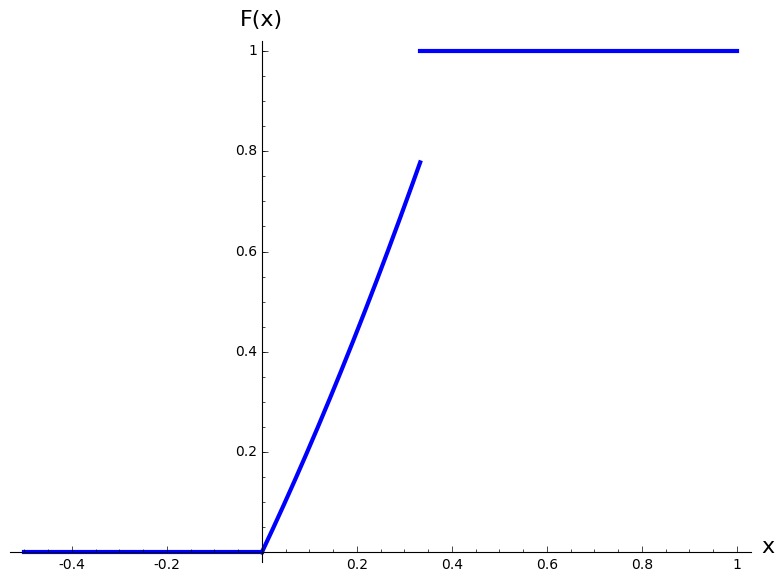
\includegraphics[width=340pt,natwidth=784,natheight=581]{4_6_1.png}
\begin{equation*}
f(x) = F^{\prime}(x) =
 \begin{cases}
  0, & x\le0\\
  6x+2, & 0<x\le\frac{1}{3}\\
  0, & x>\frac{1}{3}
 \end{cases}
\end{equation*}
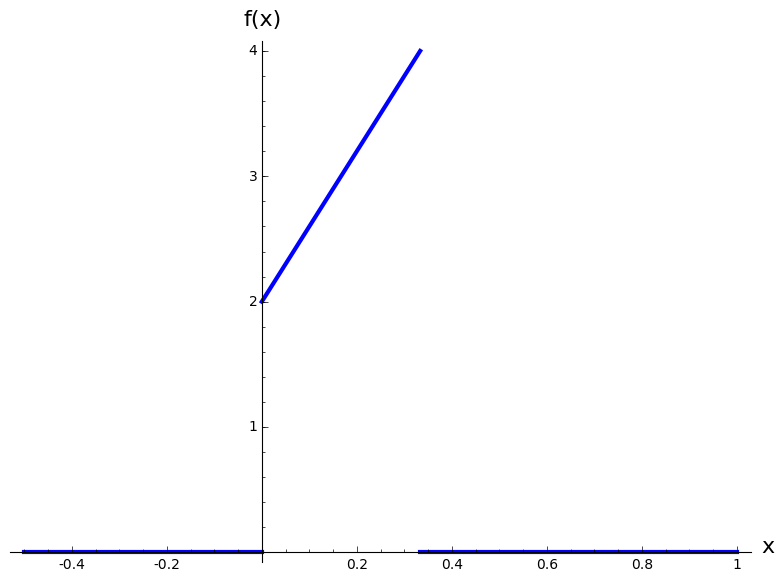
\includegraphics[width=340pt,natwidth=784,natheight=581]{4_6_2.png}
$$m=M(X)=\int_{-\infty}^{+\infty} x f(x) dx=\int_{0}^{1/3} x(6x+2) dx=\int_{0}^{1/3} 6x^2dx + \int_{0}^{1/3} 2xdx=(2x^3+x^2)\bigg|_{0}^{\frac{1}{3}}=\frac{5}{27}\approx0,185.$$
$$D(X)=\int_{-\infty}^{+\infty} (x-m)^2 f(x) dx=\int_{0}^{1/3} \left(x-\frac{5}{27}\right)^2(6x+2) dx=\int_{0}^{1/3} \left(6x^3-\frac{2x^2}{9}-\frac{130x}{243}+\frac{50}{729}\right) dx=$$
$$=\left(\frac{3x^4}{2}-\frac{2x^3}{27}-\frac{65x^2}{243}+\frac{50x}{729}\right)\bigg|_{0}^{\frac{1}{3}}=\frac{1}{54}-\frac{2}{729}-\frac{65}{2187}+\frac{50}{2187}=\frac{6,5}{729}\approx0,0089.$$

\item % Задание 7
Заданы математическое ожидание $m$ и среднее квадратическое отклонение $\sigma$ нормально распределённой случайной величины. \newline
Требуется найти: а) вероятность того, что $X$ примет значение, принадлежащее интервалу $(a, b)$; \newline
б) вероятность того, что абсолютная величина отклонения $|X-m|$ окажется меньше положительного числа $n$.

$$m=9;\sigma=5;a=5;b=15;n=8$$
\begin{center}Решение:\end{center}
а) $$P(a<X<b)=\Phi\left(\frac{b-m}{\sigma}\right)-\Phi\left(\frac{a-m}{\sigma}\right)=\Phi\left(\frac{15-9}{5}\right)-\Phi\left(\frac{5-9}{5}\right)=$$
$$=\Phi(1,2)+\Phi(0,8)=0,38493+0,28814=0,67307.$$
б)
$$P (|X-m| < n)= 2\Phi\left(\frac{n}{\sigma}\right)=2\Phi\left(\frac{8}{5}\right)=2\Phi(1,6)=2\cdot0,44520=0,8904.$$

Ответ: а)$0,67307$; б)$0,8904$.

\item % Задание 8
Дано статическое распределение выборки (в первой строке указаны выборочные варианты $x_j$, а во второй строке - соответствующие частоты).

Требуется:

1) Построить полигон частот.

2) Найти выборочнуюсреднюю $x_\textit{в}$ (несмещённую оценку средней)

3) Найти выборочную дисперсию (смещённую оценку)

4) Найти <<Исправленную>> выборочную дисперсию $S^2$ (несмещённую оценку) и <<исправленное>> среднее квадратическое отклонение $S$.

\begin{center}
\begin{tabular}{|c|c|c|c|c|c|c|c|}
\hline
$x_j$ & 130 & 140 & 160 & 170 & 190 & 200 & 220 \\
\hline
$n_j$ & 20 & 15 & 5 & 10 & 25 & 30 & 40 \\
\hline
\end{tabular}
\end{center}
\begin{center}Решение:\end{center}
1) Найдем сначала объём выборки: $$n=\sum_{j=1}^k n_j=20+15+5+10+25+30+40=145$$

Полигон частот:

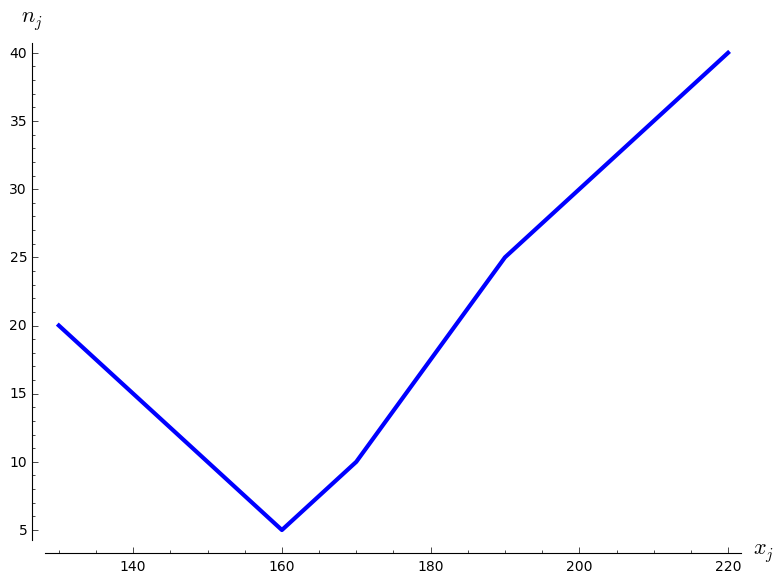
\includegraphics[width=340pt,natwidth=783,natheight=583]{4_8.png}

2) Выборочная средняя:
$$\overline{x_\textit{в}}=\frac{1}{n}\sum_{j=1}^k n_j x_j=\frac{1}{145}\cdot\left(20\cdot130+15\cdot140+5\cdot160+10\cdot170+25\cdot190+30\cdot200+40\cdot220\right)=$$
$$=\frac{26750}{145}=\frac{5350}{29}\approx184,48.$$

3) Выборочная дисперсия:
\begin{multline*}
D_{\textit{в}}=\frac{1}{n}\sum_{j=1}^k n_j
\cdot\left(x_j-\overline{x_\textit{в}}\right)^2=
\frac{1}{145}\cdot\left(20\cdot\left(130-\frac{5350}{29}\right)^2+15\cdot\left(140-\frac{5350}{29}\right)^2+5\cdot\left(160-\frac{5350}{29}\right)^2+\right.\\
+\left.10\cdot\left(170-\frac{5350}{29}\right)^2+25\cdot\left(190-\frac{5350}{29}\right)^2+30\cdot\left(200-\frac{5350}{29}\right)^2+40\cdot\left(220-\frac{5350}{29}\right)^2\right)=\\
=\frac{1}{145\cdot29^2}\cdot\left(20\cdot1580^2+15\cdot1290^2+5\cdot710^2+10\cdot420^2+25\cdot160^2+30\cdot450^2+40\cdot1030^2\right)=\\
=\frac{100}{121945}\cdot\left(20\cdot24964+15\cdot16641+5\cdot5041+10\cdot1764+25\cdot256+30\cdot2025+40\cdot10609\right)=
\end{multline*}
$$=\frac{128325000}{121945}\approx1052,3.$$
4) <<Исправленная>> выборочная дисперсия:
$$S^2=\frac{n}{n-1}D_{\textit{в}}=\frac{128325000}{144\cdot29^2}\approx1059,6.$$
<<Исправленное>> среднее квадратическое отклонение:
$$S=\sqrt{S^2}=\sqrt{\frac{128325000}{144\cdot29^2}}\approx32,55$$

\item % Задание 9
Найти доверительные интервалы для оценки математического ожидания с надёжностью $\gamma=0,95$; зная выборочную среднюю $\overline{x_\textit{в}}$, объём выборки $n$ и среднее математическое отклонение $\sigma$ нормально распределенной величины $X$.

$$\overline{x_\textit{в}}=175,41; \sigma=12; n=144.$$
\begin{center}Решение:\end{center}
$$\overline{x_\textit{в}}-t\cdot\left(\frac{\sigma}{\sqrt{n}}\right)<m<\overline{x_\textit{в}}+t\cdot\left(\frac{\sigma}{\sqrt{n}}\right)$$
Значению функции Лапласа $\Phi(t)=\frac{\gamma}{2}=\frac{0,95}{2}=0,475$ соответствует $t=1,96$.

Теперь мы знаем всё для того чтобы найти доверительный интервал для оценки математического ожидания:
$$175,41-1,96\cdot\left(\frac{12}{\sqrt{144}}\right)<m<175,41+1,96\cdot\left(\frac{12}{\sqrt{144}}\right);$$
$$175,41-1,96<m<175,41+1,96;$$
$$173,45<m<177,37.$$
Ответ: $(173,45;177,37)$.

\end{enumerate}

\section*{Вариант № 8.}
\begin{enumerate}

\item % Задание 1
В лотерее 10 билетов, из них 5 билетов выигрышных. Наудачу берётся 2 билета. Найти вероятность того, что среди них: а) оба билета выигрышные; б) хотя бы один билет выигрышный.
\begin{center}Решение:\end{center}
Перенумеруем все билеты. Исходом считаем выбор 2 любых билетов.
Количество всех исходов равно
$$n=C_{10}^{2}=\frac{10!}{2!\cdot8!}=\frac{9\cdot10}{2}=45$$
а) Благоприятный исход - выбор двух выигрышных билетов. \newline
2 выигрышных билета из 5 можно выбрать $C_{5}^{2}$ способами. \newline
Значит количество благоприятных исходов равно
$$m=C_{5}^{2}=\frac{5!}{2!\cdot3!}=\frac{4\cdot5}{2}=10$$
$$P=\frac{m}{n}=\frac{10}{45}=\frac{2}{9}\approx0,22$$
б) Неблагоприятный исход $\overline{A}$ - выбор двух проигрышных билетов.  \newline
2 проигрышных билета из 5 можно выбрать $C_{5}^{2}=10$ способами. И вероятность их выбрать такая же как при выборе двух выигрышных $P(\overline{A})=\frac{10}{45}=\frac{2}{9}$ \newline
$$P(A)=1-P(\overline{A})=1-\frac{2}{9}=\frac{7}{9}\approx0,78$$
Ответ: а) $\approx0,22$; б) $\approx0,78$.

\item % Задание 2
В ящике 40 деталей, из них 10 высшего сорта. Наудачу извлечены 2 детали. Найти вероятность того, что среди них высшего сорта: а) одна деталь; б) хотя бы одна деталь.
\begin{center}Решение:\end{center}
Перенумеруем все детали. Исходом считаем выбор 2 любых деталей.
Количество всех исходов равно
$$n=C_{40}^{2}=\frac{40!}{2!\cdot38!}=\frac{40\cdot39}{2}=780$$
а) Благоприятный исход - выбор одной детали высшего сорта и другой не высшего. \newline
1 деталь высшего сорта из 10 можно выбрать $10$ способами. А выбрать одну деталь не высшего сорта из 30 можно $30$ способами. \newline
Количество благоприятных исходов равно произведению
$$m=10\cdot30=300$$
$$P=\frac{m}{n}=\frac{300}{780}=\frac{5}{13}\approx0,38$$
б) Неблагоприятный исход $\overline{A}$ - выбор обеих деталей не высшего сорта.
Две детали не высшего сорта из 30 можно выбрать $C_{30}^{2}$ способами.
$$m_1=C_{30}^{2}=\frac{30!}{2!\cdot28!}=\frac{29\cdot30}{2}=29\cdot15=435$$
$$P(\overline{A})=\frac{m_1}{n}=\frac{435}{780}\approx0,56$$
$$P(A)=1-P(\overline{A})\approx0,44$$
Ответ: а) $\approx0,38$; б) $\approx0,44$.

\item % Задание 3
Из ста деталей 60 первого, 30 второго и 10 третьего сорта. Вероятность брака среди деталей первого, второго и третьего сорта соответственно равна $0,01$, $0,03$ и $0,05$. Наудачу взятая деталь оказалась небракованной. Найти вероятность того, что взятая деталь первого сорта.
\begin{center}Решение:\end{center}
Всего у нас $60+30+10=100$ деталей.  \newline
Пусть $H_1$,$H_2$,$H_3$ - гипотезы о том, что наудачу взятая деталь имеет соответственно первый, второй и третий сорт. \newline Тогда по формуле классической вероятности находим априорные вероятности $P(H_1)=\frac{60}{100}=0,6$; $P(H_2)=\frac{30}{100}=0,3$; $P(H_3)=\frac{10}{100}=0,1$.  \newline Пусть событие $A$ состоит в том, что деталь оказалась небракованной. Далее из условия находим:  \newline $P(A/H_1)=1-P(\overline{A}/H_1)=1-0,01=0,99$,  \newline $P(A/H_2)=1-P(\overline{A}/H_2)=1-0,03=0,97$,  \newline $P(A/H_3)=1-P(\overline{A}/H_3)=1-0,05=0,95$.  \newline Теперь для нахождения искомой $P(H_1/A)$ можно применить формулу Байеса:

$$P(H_1/A)=\frac{P(H_1)P(A/H_1)}{P(H_1)P(A/H_1)+P(H_2)P(A/H_2)+P(H_3)P(A/H_3)}=$$
$$=\frac{0,6\cdot0,99}{0,6\cdot0,99+0,3\cdot0,97+0,1\cdot0,95}=
\frac{0,594}{0,98}\approx0,6.$$

Ответ: $\approx0,6$.

\item % Задание 4
Найти вероятность того, что в $n$ независимых испытаний событие появится не менее $k$ раз, зная, что в каждом испытании вероятность появления события равна $p$.

$$n=6; k=4; p=0,8.$$
\begin{center}Решение:\end{center}
Используем формулу Бернулли $P_n(k)=C_n^k p^k q^{n-k}$, вероятность того, что событие наступит не менее $k$ раз с помощью неё вычисляется так: $$P_n(i\ge k)=\sum_{i=k}^n P_n(i)$$
В нашем случае $n=6; k=4; p=0,8; q=0,2;$ значит
$$P_6(i\ge 4)=\sum_{i=4}^6 P_6(i)=P_6(4)+P_6(5)+P_6(6)=C_6^4\cdot0,8^4\cdot0,2^2+C_6^5\cdot0,8^5\cdot0,2+C_6^6\cdot0,8^6=$$
$$=15\cdot0,4096\cdot0,04+6\cdot0,32768\cdot0,2+0,262144=0,24576+0,393216+0,262144=0,90112.$$

Ответ: $0,90112$.

\item % Задание 5
Найти а) математическое ожидание; б) дисперсию; в) среднее квадратическое отклонение дискретной случайной величины $X$ по закону её распределения, заданному рядом распределения (в первой строке таблицы указаны возможные значения, во второй строке - вероятности возможных значений).

\begin{center}
\begin{tabular}{|c|c|c|c|c|c|}
\hline
$X$ & 115 & 135 & 150 & 175 & 180 \\
\hline
$p$ & $0,1$ & $0,5$ & $0,2$ & $0,1$ & $0,1$ \\
\hline
\end{tabular}
\end{center}
\begin{center}Решение:\end{center}
а) Математическое ожидание: $$M(X)=\sum_{i=1}^n x_i p_i=115\cdot0,1+135\cdot0,5+150\cdot0,2+175\cdot0,1+180\cdot0,1=11,5+67,5+30+17,5+18=144,5.$$
б) Дисперсия:
$$D(X)=\sum_{i=1}^n (x_i-m)^2 p_i=(115-144,5)^2\cdot0,1+(135-144,5)^2\cdot0,5+(150-144,5)^2\cdot0,2+(175-144,5)^2\cdot0,1+$$
$$+(180-144,5)^2\cdot0,1=29,5^2\cdot0,1+9,5^2\cdot0,5+5,5^2\cdot0,2+30,5^2\cdot0,1+35,5^2\cdot0,1=357,25.$$
в) Среднее квадратическое отклонение:
$$\sigma=\sqrt{D(X)}=\sqrt{357,25}\approx18,9.$$

Ответ: а)$144,5$; б)$357,25$; в)$\approx18,9$.

\item % Задание 6
Случайная величина $X$ задана функцией распределения $F(x)$. Найти плотность распределения вероятностей, математическое ожидание, дисперсию случайной величины и построить графики $f(x)$ и $F(x)$.

\begin{equation*}
F(x) =
 \begin{cases}
  0, & x\leq-\pi/2\\
  \cos{x}, & -\pi/2<x\le0\\
  1, & x>0
 \end{cases}
\end{equation*}
\begin{center}Решение:\end{center}
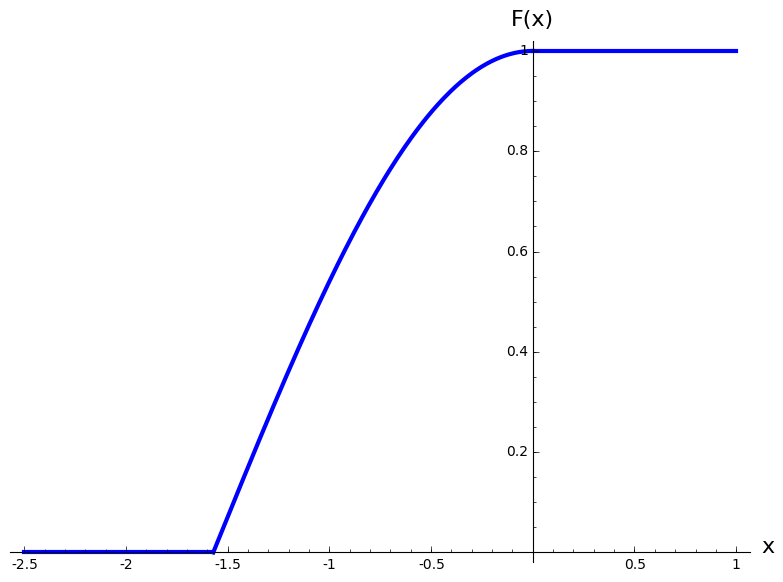
\includegraphics[width=340pt,natwidth=784,natheight=581]{8_6_1.png}
\begin{equation*}
f(x) = F^{\prime}(x) =
 \begin{cases}
  0, & x\le-\pi/2\\
  -\sin{x}, & -\pi/2<x\le0\\
  0, & x>0
 \end{cases}
\end{equation*}
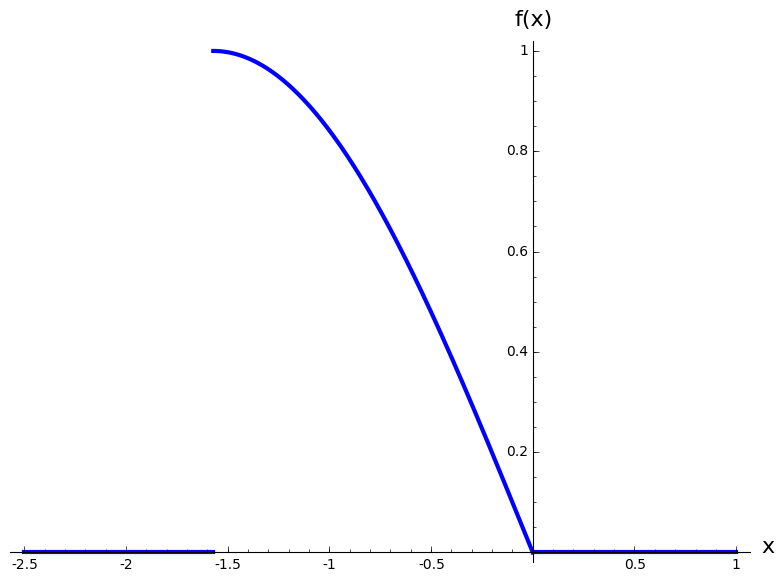
\includegraphics[width=340pt,natwidth=784,natheight=581]{8_6_2.png}
$$m=M(X)=\int_{-\infty}^{+\infty} x f(x) dx=\int_{-\frac{\pi}{2}}^{0} \left(-x\sin{x}\right) dx=\left\langle \begin{array}{cc} u=x & du=dx \\ -\sin{x}dx=dv & v=\cos{x} \end{array} \right\rangle=$$ $$=x\cos{x}\bigg|_{-\frac{\pi}{2}}^{0}-\int_{-\frac{\pi}{2}}^{0} \cos{x} dx=\left(x\cos{x}-\sin{x}\right)\bigg|_{-\frac{\pi}{2}}^{0}=
\left(0\cos{0}-\sin{0}\right)-\left(-\frac{\pi}{2}\cos{\left(-\frac{\pi}{2}\right)}-\left(\sin{\left(-\frac{\pi}{2}\right)}\right)\right)=-1.$$

$$D(X)=\int_{-\infty}^{+\infty} (x-m)^2 f(x) dx=\int_{-\frac{\pi}{2}}^{0} \left(x+1\right)^2(-\sin{x}) dx
=\int_{-\frac{\pi}{2}}^{0} \left(x^2+2x+1\right)(-\sin{x}) dx=-\int_{-\frac{\pi}{2}}^{0} x^2\sin{x} dx-$$
$$-2\int_{-\frac{\pi}{2}}^{0} x\sin{x} dx-\int_{-\frac{\pi}{2}}^{0} \sin{x} dx=-\int_{-\frac{\pi}{2}}^{0} x^2\sin{x} dx-2+\cos{x}\bigg|_{-\frac{\pi}{2}}^{0}=-1-\int_{-\frac{\pi}{2}}^{0} x^2\sin{x} dx=$$
$$=\left\langle \begin{array}{cc} u=x^2 & du=2xdx \\ -\sin{x}dx=dv & v=\cos{x} \end{array} \right\rangle=-1+x^2\cos{x}\bigg|_{-\frac{\pi}{2}}^{0}-\int_{-\frac{\pi}{2}}^{0}\cos{x}\cdot2xdx=-1-2\int_{-\frac{\pi}{2}}^{0}x\cos{x}dx=$$
$$=\left\langle \begin{array}{cc} u=x & du=dx \\ cos{x}dx=dv & v=\sin{x} \end{array} \right\rangle=-1-2x\sin{x}\bigg|_{-\frac{\pi}{2}}^{0}+2\int_{-\frac{\pi}{2}}^{0}\sin{x}dx=-1-2x\sin{x}\bigg|_{-\frac{\pi}{2}}^{0}-2\cos{x}\bigg|_{-\frac{\pi}{2}}^{0}=$$
$$=-1-2\cdot0\sin{0}+2\left(-\frac{\pi}{2}\right)\sin{\left(-\frac{\pi}{2}\right)}-2\cos{0}+2\cos{\left(-\frac{\pi}{2}\right)}=\pi-3\approx0,14.$$

\item % Задание 7
Заданы математическое ожидание $m$ и среднее квадратическое отклонение $\sigma$ нормально распределённой случайной величины. \newline
Требуется найти: а) вероятность того, что $X$ примет значение, принадлежащее интервалу $(a, b)$; \newline
б) вероятность того, что абсолютная величина отклонения $|X-m|$ окажется меньше положительного числа $n$.

$$m=13;\sigma=3;a=9;b=19;n=4$$
\begin{center}Решение:\end{center}
а) $$P(a<X<b)=\Phi\left(\frac{b-m}{\sigma}\right)-\Phi\left(\frac{a-m}{\sigma}\right)=\Phi\left(\frac{19-13}{3}\right)-\Phi\left(\frac{9-13}{3}\right)=$$
$$=\Phi(2)+\Phi\left(\frac{4}{3}\right)=0,47725+0,40824=0,88549.$$
б)
$$P (|X-m| < n)= 2\Phi\left(\frac{n}{\sigma}\right)=2\Phi\left(\frac{4}{3}\right)=2\cdot0,40824=0,81648.$$

Ответ: а)$0,88549$; б)$0,81648$.

\item % Задание 8
Дано статическое распределение выборки (в первой строке указаны выборочные варианты $x_j$, а во второй строке - соответствующие частоты).

Требуется:

1) Построить полигон частот.

2) Найти выборочнуюсреднюю $x_\textit{в}$ (несмещённую оценку средней)

3) Найти выборочную дисперсию (смещённую оценку)

4) Найти <<Исправленную>> выборочную дисперсию $S^2$ (несмещённую оценку) и <<исправленное>> среднее квадратическое отклонение $S$.

\begin{center}
\begin{tabular}{|c|c|c|c|c|c|c|c|}
\hline
$x_j$ & 100 & 110 & 150 & 170 & 180 & 200 & 220 \\
\hline
$n_j$ & 5 & 10 & 20 & 30 & 15 & 25 & 40 \\
\hline
\end{tabular}
\end{center}
\begin{center}Решение:\end{center}
1) Найдем сначала объём выборки: $$n=\sum_{j=1}^k n_j=5+10+20+30+15+25+40=145$$

Полигон частот:

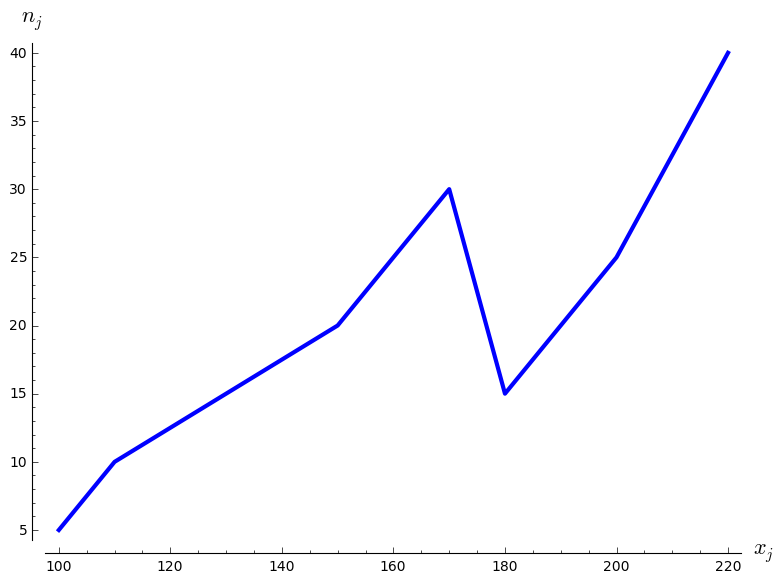
\includegraphics[width=340pt,natwidth=783,natheight=583]{8_8.png}

2) Выборочная средняя:
$$\overline{x_\textit{в}}=\frac{1}{n}\sum_{j=1}^k n_j x_j=\frac{1}{145}\cdot\left(5\cdot100+10\cdot110+20\cdot150+30\cdot170+15\cdot180+25\cdot200+40\cdot220\right)=$$
$$=\frac{26200}{145}=\frac{5240}{29}\approx180,69.$$

3) Выборочная дисперсия:
\begin{multline*}
D_{\textit{в}}=\frac{1}{n}\sum_{j=1}^k n_j
\cdot\left(x_j-\overline{x_\textit{в}}\right)^2=
\frac{1}{145}\cdot\left(5\cdot\left(100-\frac{5240}{29}\right)^2+10\cdot\left(110-\frac{5240}{29}\right)^2+20\cdot\left(150-\frac{5240}{29}\right)^2+\right.\\
+\left.30\cdot\left(170-\frac{5240}{29}\right)^2+15\cdot\left(180-\frac{5240}{29}\right)^2+25\cdot\left(200-\frac{5240}{29}\right)^2+40\cdot\left(220-\frac{5240}{29}\right)^2\right)=\\
=\frac{1}{145\cdot29^2}\cdot\left(5\cdot2340^2+10\cdot2050^2+20\cdot890^2+30\cdot310^2+15\cdot20^2+25\cdot560^2+40\cdot1140^2\right)=\\
=\frac{100}{121945}\cdot\left(5\cdot54756+10\cdot42025+20\cdot7921+30\cdot961+15\cdot4+25\cdot3136+40\cdot12996\right)=
\end{multline*}
$$=\frac{147958000}{121945}\approx1213,3.$$
4) <<Исправленная>> выборочная дисперсия:
$$S^2=\frac{n}{n-1}D_{\textit{в}}=\frac{147958000}{144\cdot29^2}\approx1221,74.$$
<<Исправленное>> среднее квадратическое отклонение:
$$S=\sqrt{S^2}=\sqrt{\frac{147958000}{144\cdot29^2}}\approx34,95$$

\item % Задание 9
Найти доверительные интервалы для оценки математического ожидания с надёжностью $\gamma=0,95$; зная выборочную среднюю $\overline{x_\textit{в}}$, объём выборки $n$ и среднее математическое отклонение $\sigma$ нормально распределенной величины $X$.

$$\overline{x_\textit{в}}=186,06; \sigma=10; n=121.$$
\begin{center}Решение:\end{center}
$$\overline{x_\textit{в}}-t\cdot\left(\frac{\sigma}{\sqrt{n}}\right)<m<\overline{x_\textit{в}}+t\cdot\left(\frac{\sigma}{\sqrt{n}}\right)$$
Значению функции Лапласа $\Phi(t)=\frac{\gamma}{2}=\frac{0,95}{2}=0,475$ соответствует $t=1,96$.

Теперь мы знаем всё для того чтобы найти доверительный интервал для оценки математического ожидания:
$$186,06-1,96\cdot\left(\frac{10}{\sqrt{121}}\right)<m<186,06+1,96\cdot\left(\frac{10}{\sqrt{121}}\right);$$
$$186,06-\frac{19,6}{11}<m<186,06+\frac{19,6}{11};$$
$$186,06-1,78<m<186,06+1,78;$$
$$184,28<m<187,84.$$
Ответ: $(184,28;187,84)$.

\end{enumerate}

\end{document}
